\level{1}{Descrizione generale dei prodotti}
    Riportiamo di seguito una descrizione generale dei prodotti. Per una descrizione più dettagliata delle funzionalità dei prodotti, si rimanda al documento \insdoc{Analisi dei Requisiti 3.00}.

    \level{2}{Norris}
        Norris è un framework per Node.js che permette di raccogliere dati provenienti da sorgenti arbitrarie e visualizzarli come grafici in modo semplice e veloce. In particolare mette a disposizione dei suoi utenti due interfacce:
        \begin{itemize}
            \item le API interne (lato server);
            \item le API esterne (lato client).
        \end{itemize}
        
        \level{3}{API interne}
        Tramite le API interne, uno sviluppatore può creare quattro tipologie di grafici: bar chart, line chart, map chart e table. Per ogni grafico può configurare le relative impostazioni e può impostare il metodo di aggiornamento dei dati del grafico stesso. L'aggiornamento dei grafici può essere di tre tipologie, a seconda del tipo di grafico:
        \begin{itemize}
            \item in place, supportato da tutti i tipi di chart;
            \item stream, supportato da bar chart, line chart e table;
            \item movie, supportato da map chart.
        \end{itemize}
        
        Lo sviluppatore può, inoltre, scegliere di incapsulare alcuni grafici all'interno di una o più pagine web. Le API interne permettono infatti di aggiungere i grafici creati ad una o più pagine web, le quali verranno create in automatico da Norris. Lo sviluppatore, oltre a poter scegliere quali grafici inserire in queste pagine, può configurare le impostazioni di ciascuna di esse. Tra le impostazioni principali ci sono la scelta del titolo e del template della pagina.\\
        Infine, se lo sviluppatore non vuole rendere pubblici i propri grafici, può definire una funzione login, una funzione islogged e una funzione di logout. Queste verranno eseguite ogni qualvolta venga richiesto di accedere alle informazioni di un grafico.
       
        \level{3}{API esterne}
            Tramite le API esterne, un utente lato client può effettuare l'autenticazione ad un'istanza di Norris esistente e richiedere al server le informazioni inerenti ai grafici presenti in quell'istanza. In particolare l'utente client può richiedere la lista dei grafici presenti nell'istanza, nonché le informazioni di ogni singolo grafico della lista. Le informazioni verranno fornite in formato JSON.

    \level{2}{Chuck}
        Chuck, acronimo di Chart Universal Creator Kit, è una libreria JavaScript lato client che permette di incapsulare un grafico (creato tramite le API interne di Norris) all'interno di una pagina web diversa da quelle create di default da Norris. In particolare lo sviluppatore lato client deve autenticarsi ad un'istanza di Norris, richiedere un grafico e scegliere il tag HTML in cui inserire il grafico. È possibile, inoltre, modificare alcune impostazioni relative al grafico.
    
    \level{2}{Applicazione Android}
        L'applicazione Android permette di visualizzare i grafici di un'istanza di Norris da uno smartphone Android. Essa permette di scegliere l'istanza di Norris alla quale connettersi tramite autenticazione. Una volta autenticato, l'utente può visualizzare la lista di grafici esistenti e i grafici stessi.
    \level{2}{Dashboard APS}
        La dashboard rappresenta un caso d'uso di \projectname{}. In particolare, essa è un'applicazione web utile alla visualizzazione di informazioni riguardanti le linee degli autobus dell'APS di Padova, con aggiornamento real-time.\\
        Attraverso l'uso di una mappa, l'utente finale potrà vedere gli spostamenti, in tempo reale, dei mezzi di trasporto della rete urbana.\\
    
        
\level{1}{Descrizione delle interazioni che i prodotti hanno tra di loro}
    \level{2}{Norris - Chuck}
        Norris e Chuck interagiscono tramite le API esterne, le quali fungono da interfaccia tra server e client. In particolare si possono avere 3 tipologie di interazione:
        \begin{itemize}
            \item autenticazione: precede l'invio di informazioni inerenti un grafico. Chuck manda a Norris l'indirizzo dell'istanza a cui si vuole connettere, assieme ad username e password. Norris controlla se i dati inviati sono corretti e, in caso affermativo, esegue l'autenticazione. Riportiamo di seguito un diagramma esplicativo:
        	\begin{figure}[H]\centering
        		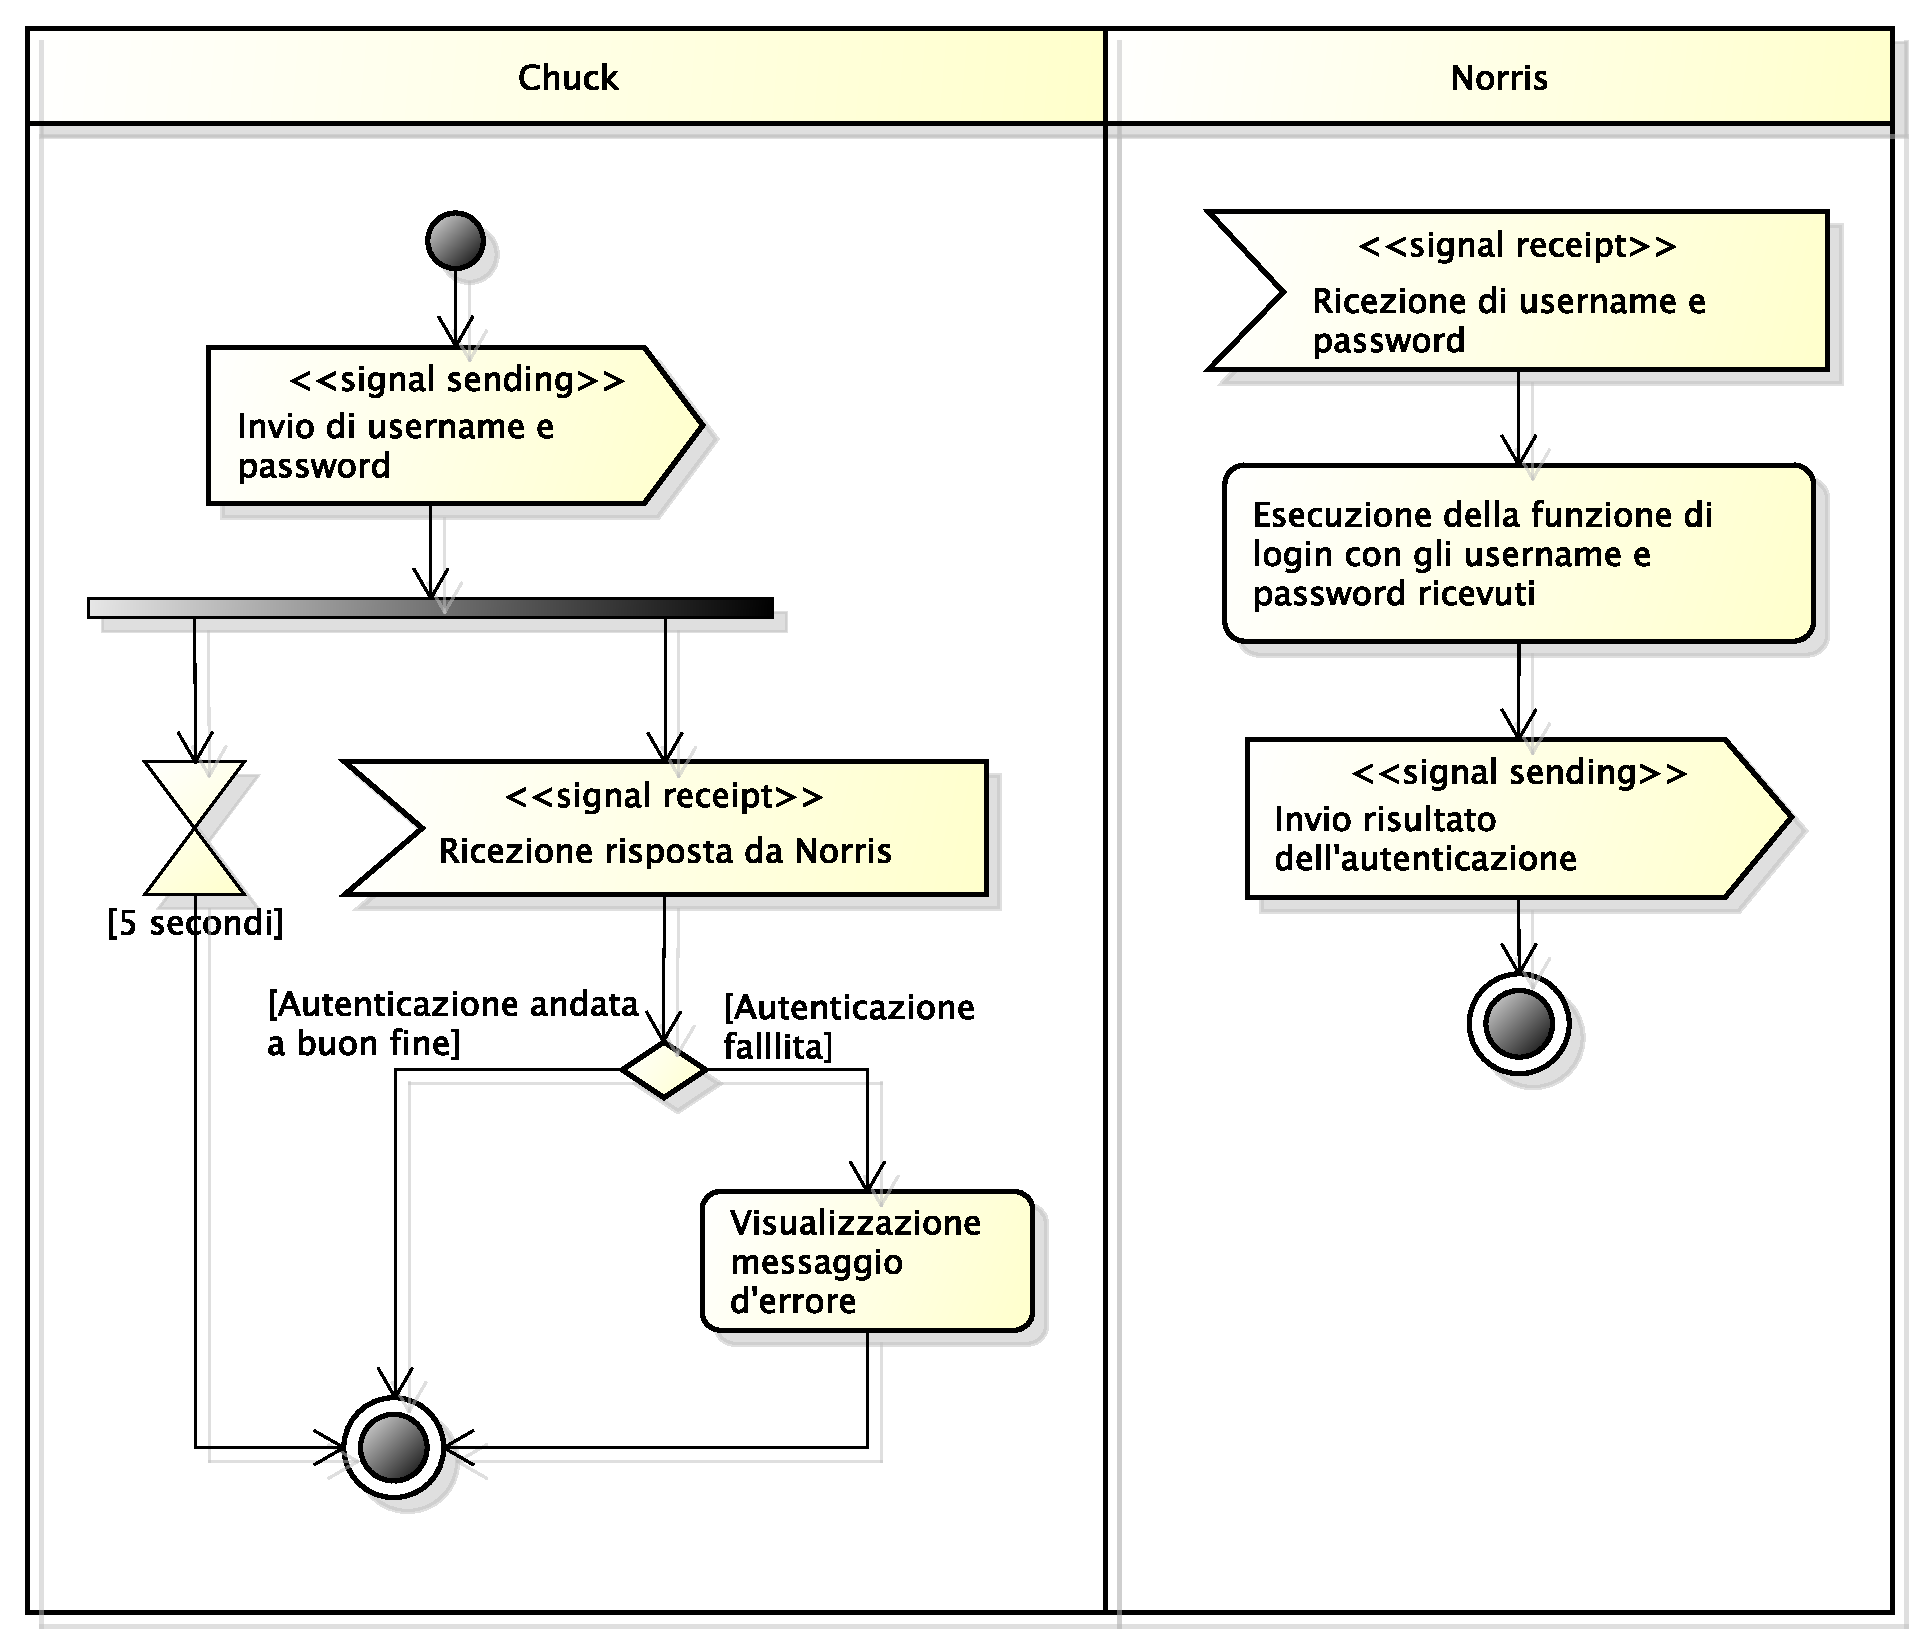
\includegraphics[width=\textwidth]{SpecificaTecnica/Pics/Chuck/Autenticazione.pdf}
        		\caption{Diagramma di attività dell'autenticazione}
    		\end{figure}
	
            \item richiesta inserimento grafico: Chuck manda a Norris una richiesta di informazioni inerenti al grafico che si vuole inserire nella pagina web. Norris controlla se il client è autenticato. In caso negativo, Norris manda una richiesta di autenticazione al client. In caso affermativo, invece, Norris manda le informazioni relative al grafico richiesto aprendo una comunicazione tramite websocket. Il canale rimane aperto fintanto che il client rimane connesso. Riportiamo di seguito un diagramma esplicativo:
            \begin{figure}[H]\centering
        	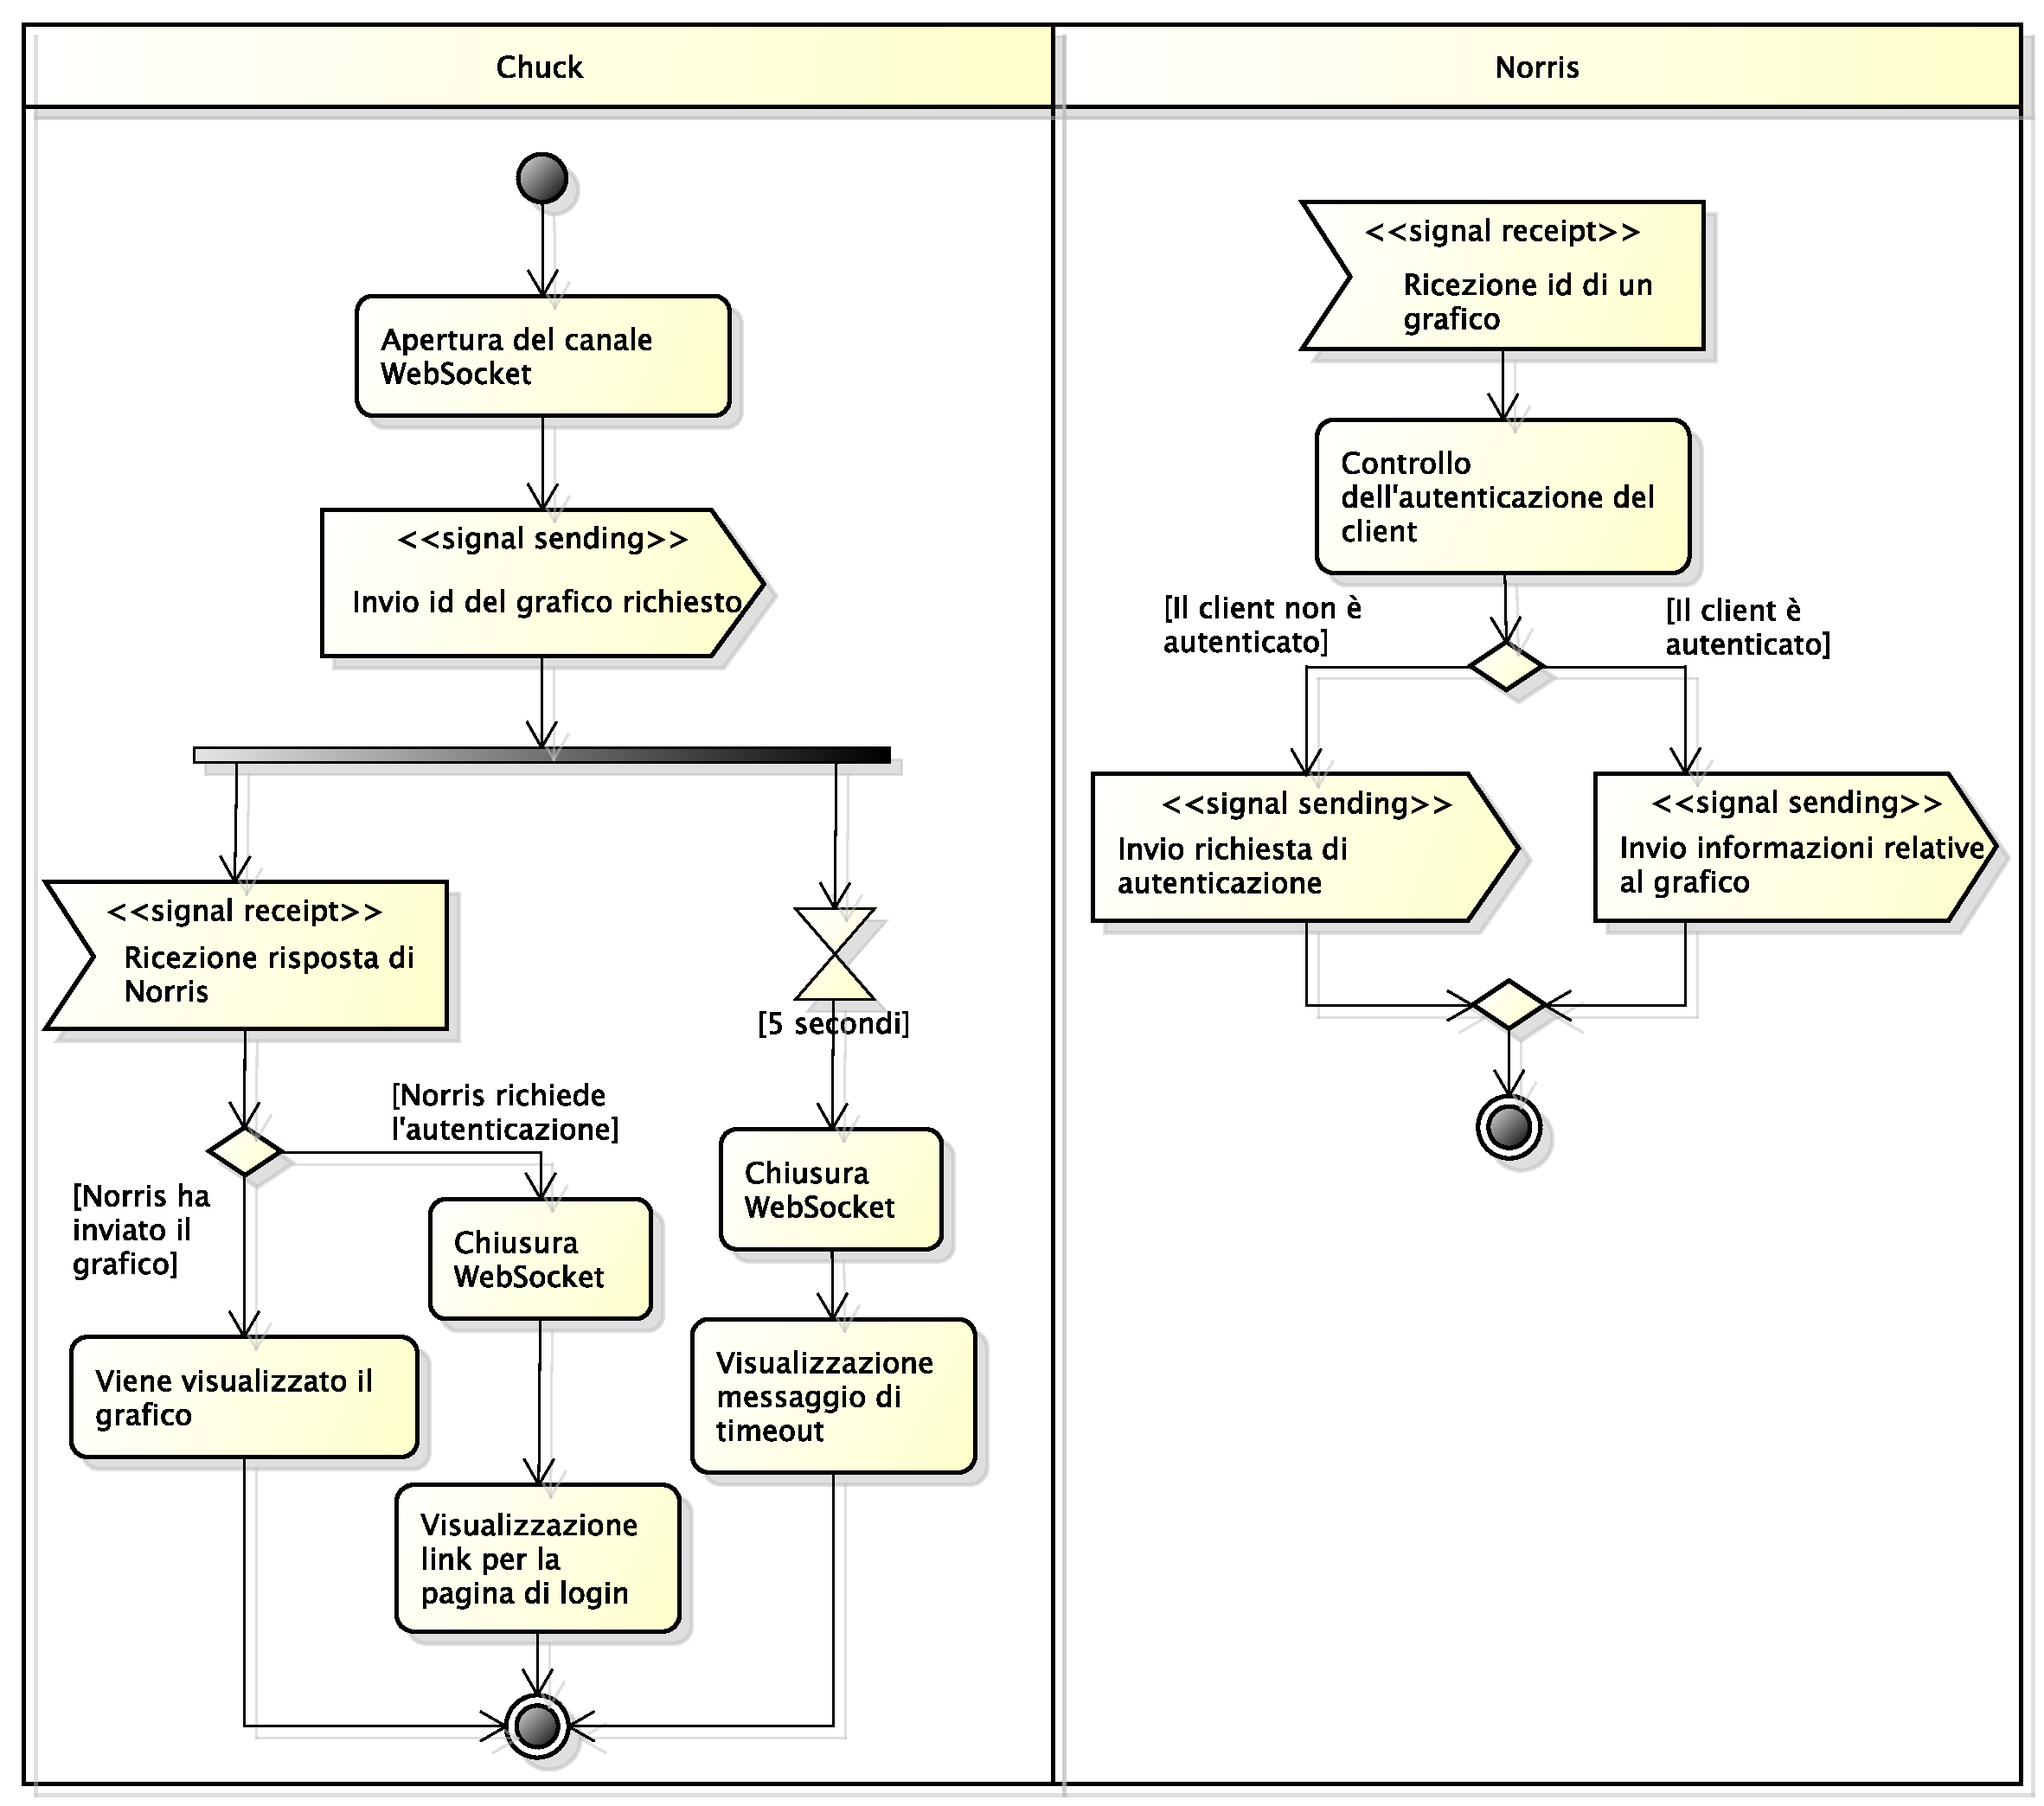
\includegraphics[width=\textwidth]{SpecificaTecnica/Pics/Chuck/RichiestaGrafico.pdf}
        	\caption{Diagramma di attività della richiesta di inserimento di un grafico}
    		\end{figure}
            \item aggiornamenti del grafico: quando un grafico viene aggiornato lato server, Norris si preoccupa di mandare l'aggiornamento ai client che hanno quel grafico. La comunicazione dell'aggiornamento avviene tramite un canale websocket appositamente creato al momento della richiesta di inserimento del grafico nella pagina web. Riportiamo di seguito un diagramma esplicativo:
            \begin{figure}[H]\centering
        	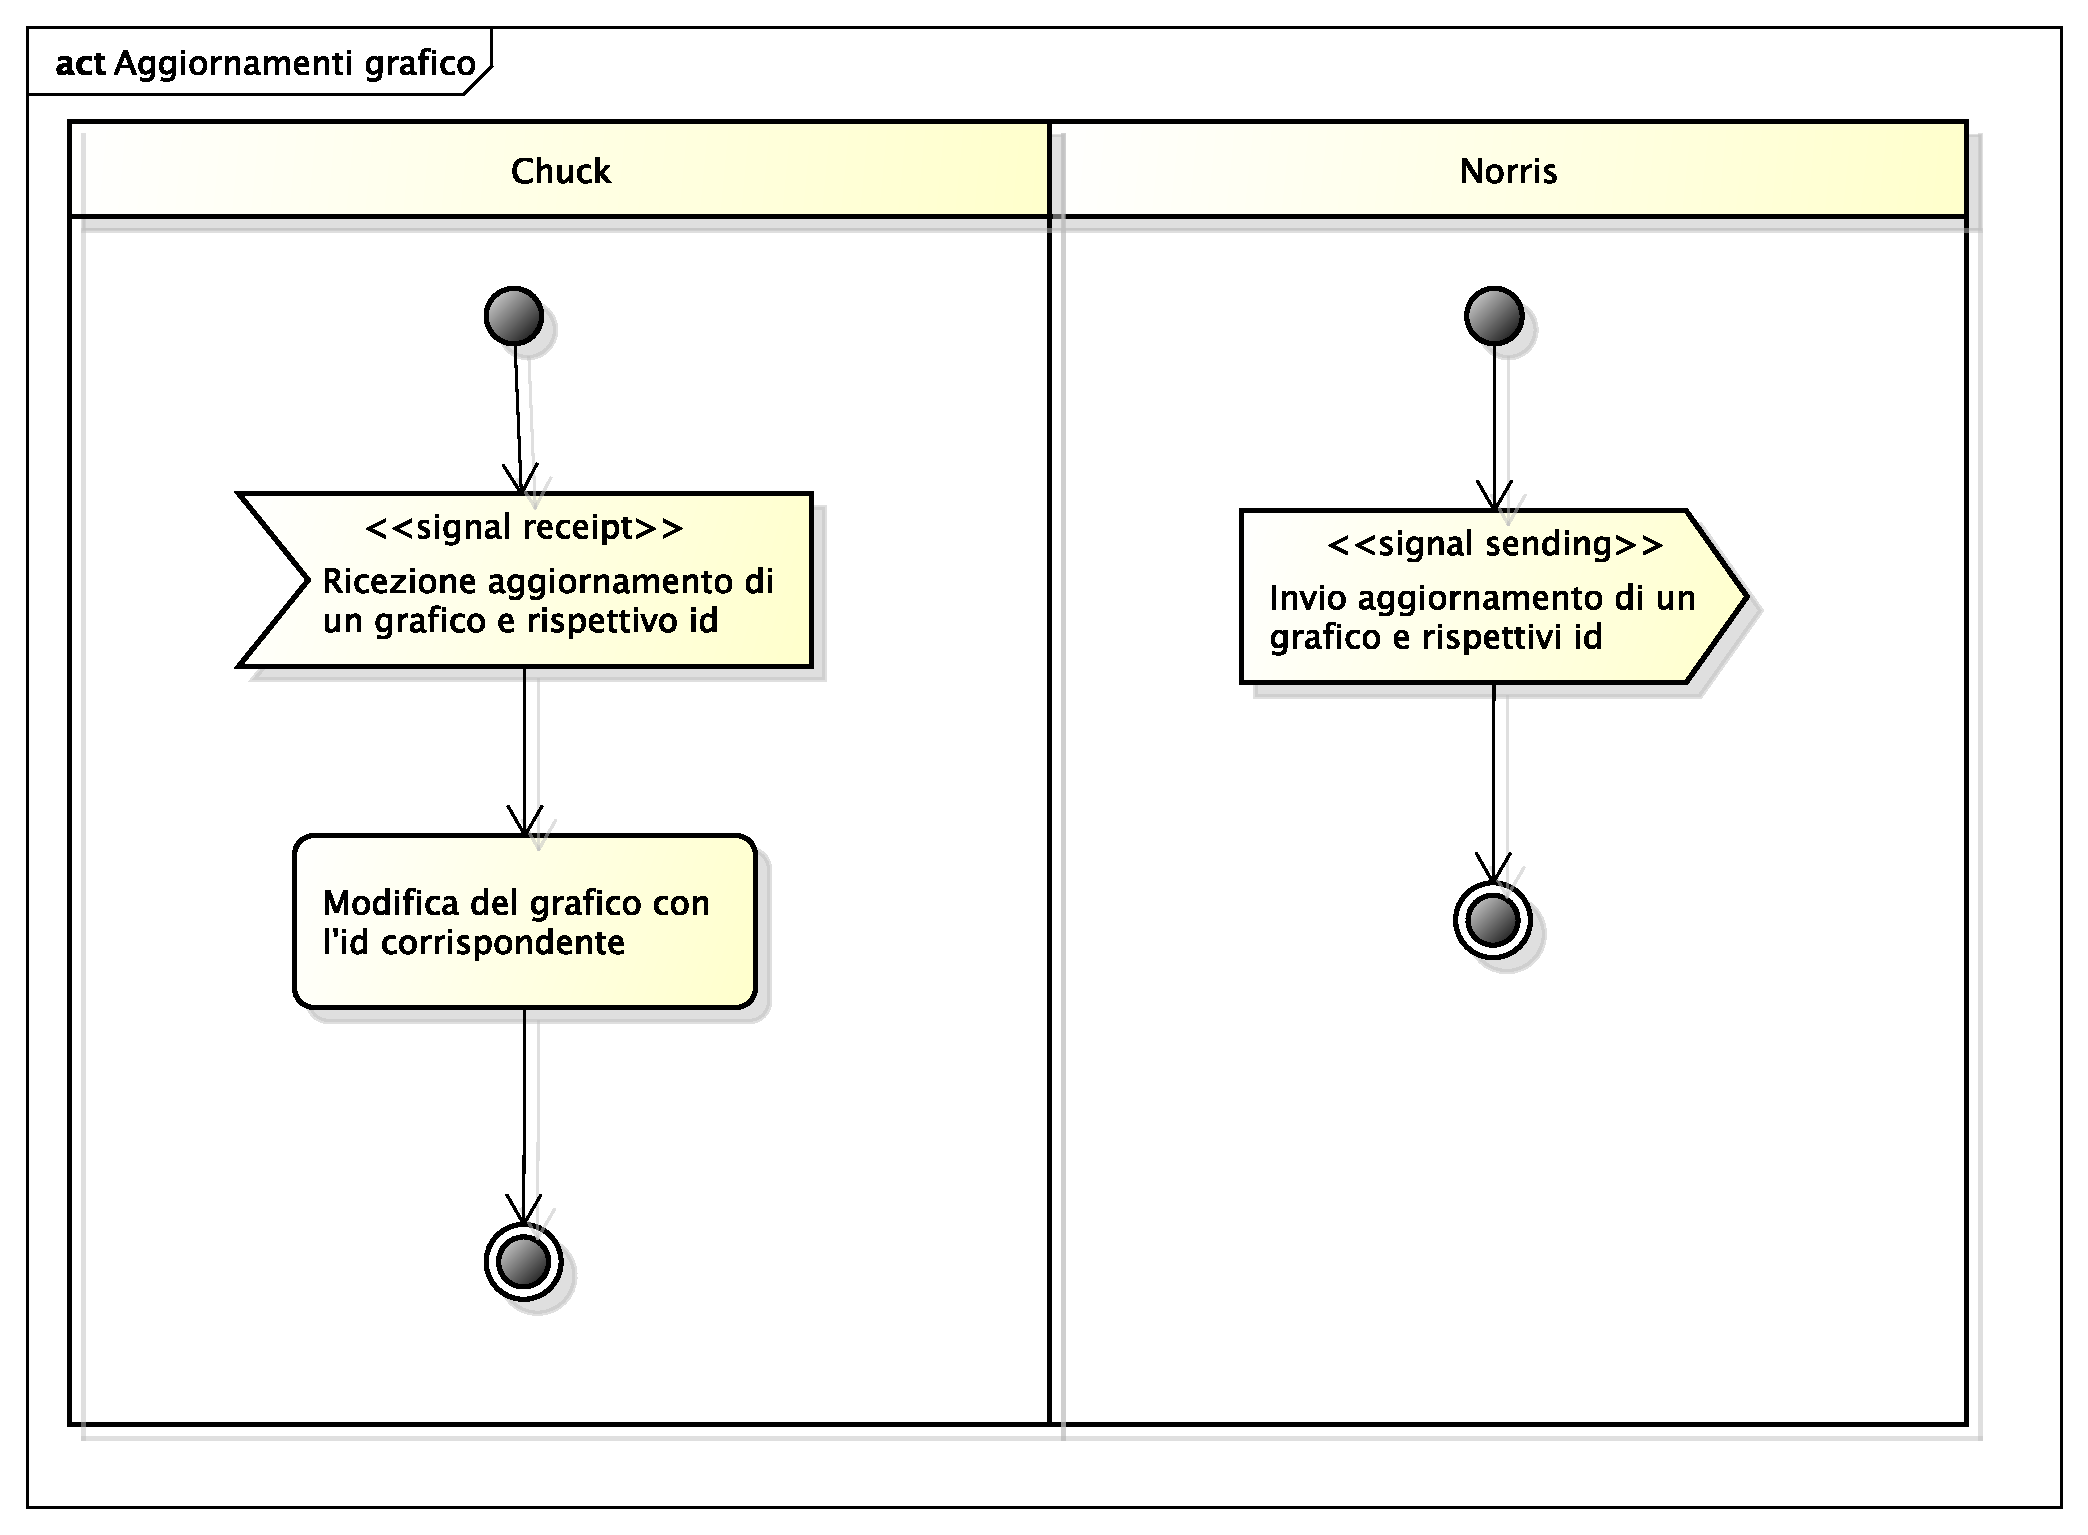
\includegraphics[width=\textwidth]{SpecificaTecnica/Pics/Chuck/AggiornamentiGrafico.pdf}
        	\caption{Diagramma di attività dell'aggiornamento di un grafico}
    		\end{figure}
        \end{itemize}
    
    \level{2}{Norris - Applicazione Android}
        Norris e l'applicazione Android interagiscono tramite le API esterne, le quali fungono da interfaccia tra server e client. In particolare si possono avere 4 tipologie di interazione:
        \begin{itemize}
            \item Autenticazione: precede l'invio di informazioni inerenti un grafico. L'applicazione Android manda a Norris l'indirizzo dell'istanza a cui si vuole connettere, assieme ad username e password. Norris controlla se i dati inviati sono corretti e, in caso affermativo, esegue l'autenticazione. Se l'autenticazione non va a buon fine, l'applicazione Android mostra un messaggio d'errore. Riportiamo di seguito un diagramma esplicativo:
        	\begin{figure}[H]\centering
        		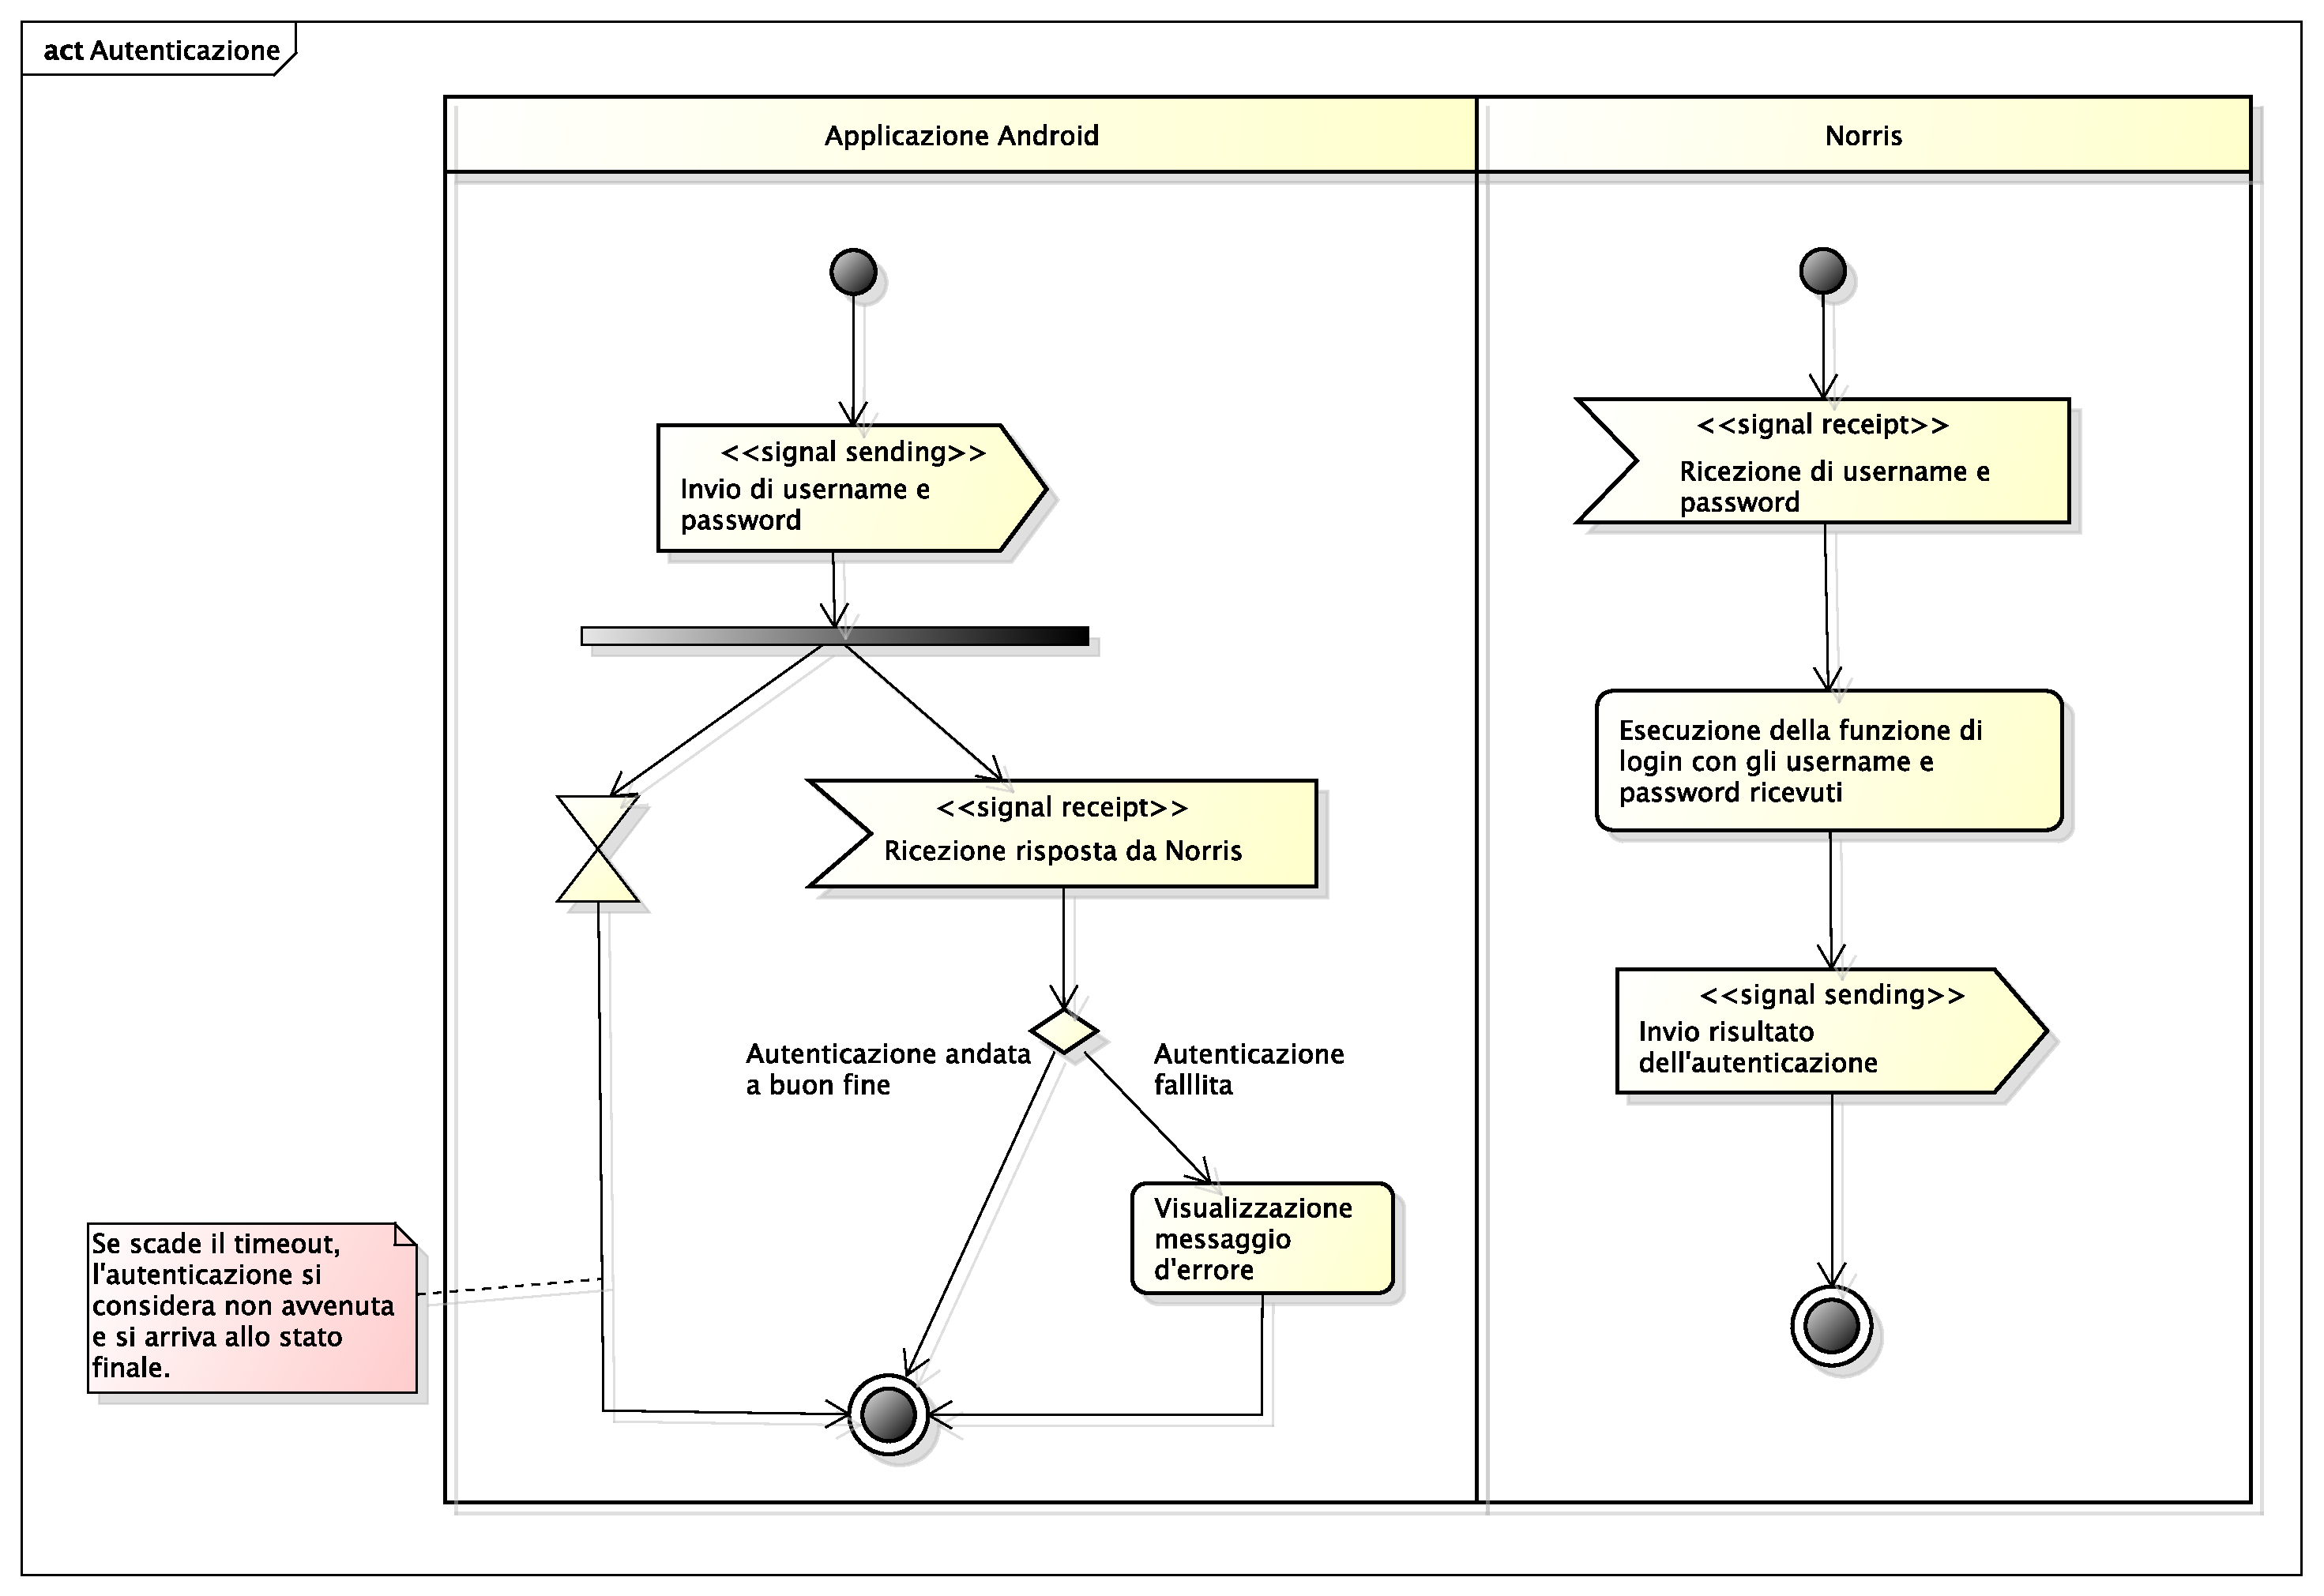
\includegraphics[width=\textwidth]{SpecificaTecnica/Pics/Applicazione/Autenticazione.pdf}
        		\caption{Diagramma di attività dell'autenticazione}
    		\end{figure}
            \item Richiesta informazioni della lista di grafici: l'applicazione Android manda a Norris una richiesta di informazioni inerenti alla lista di grafici presenti nell'istanza di Norris alla quale ci si è autenticati. Norris controlla se l'utente è autenticato e, in caso affermativo, manda le informazioni relative alla lista di grafici richiesta tramite una richiesta HTTP. Riportiamo di seguito un diagramma esplicativo:
            \begin{figure}[H]\centering
        	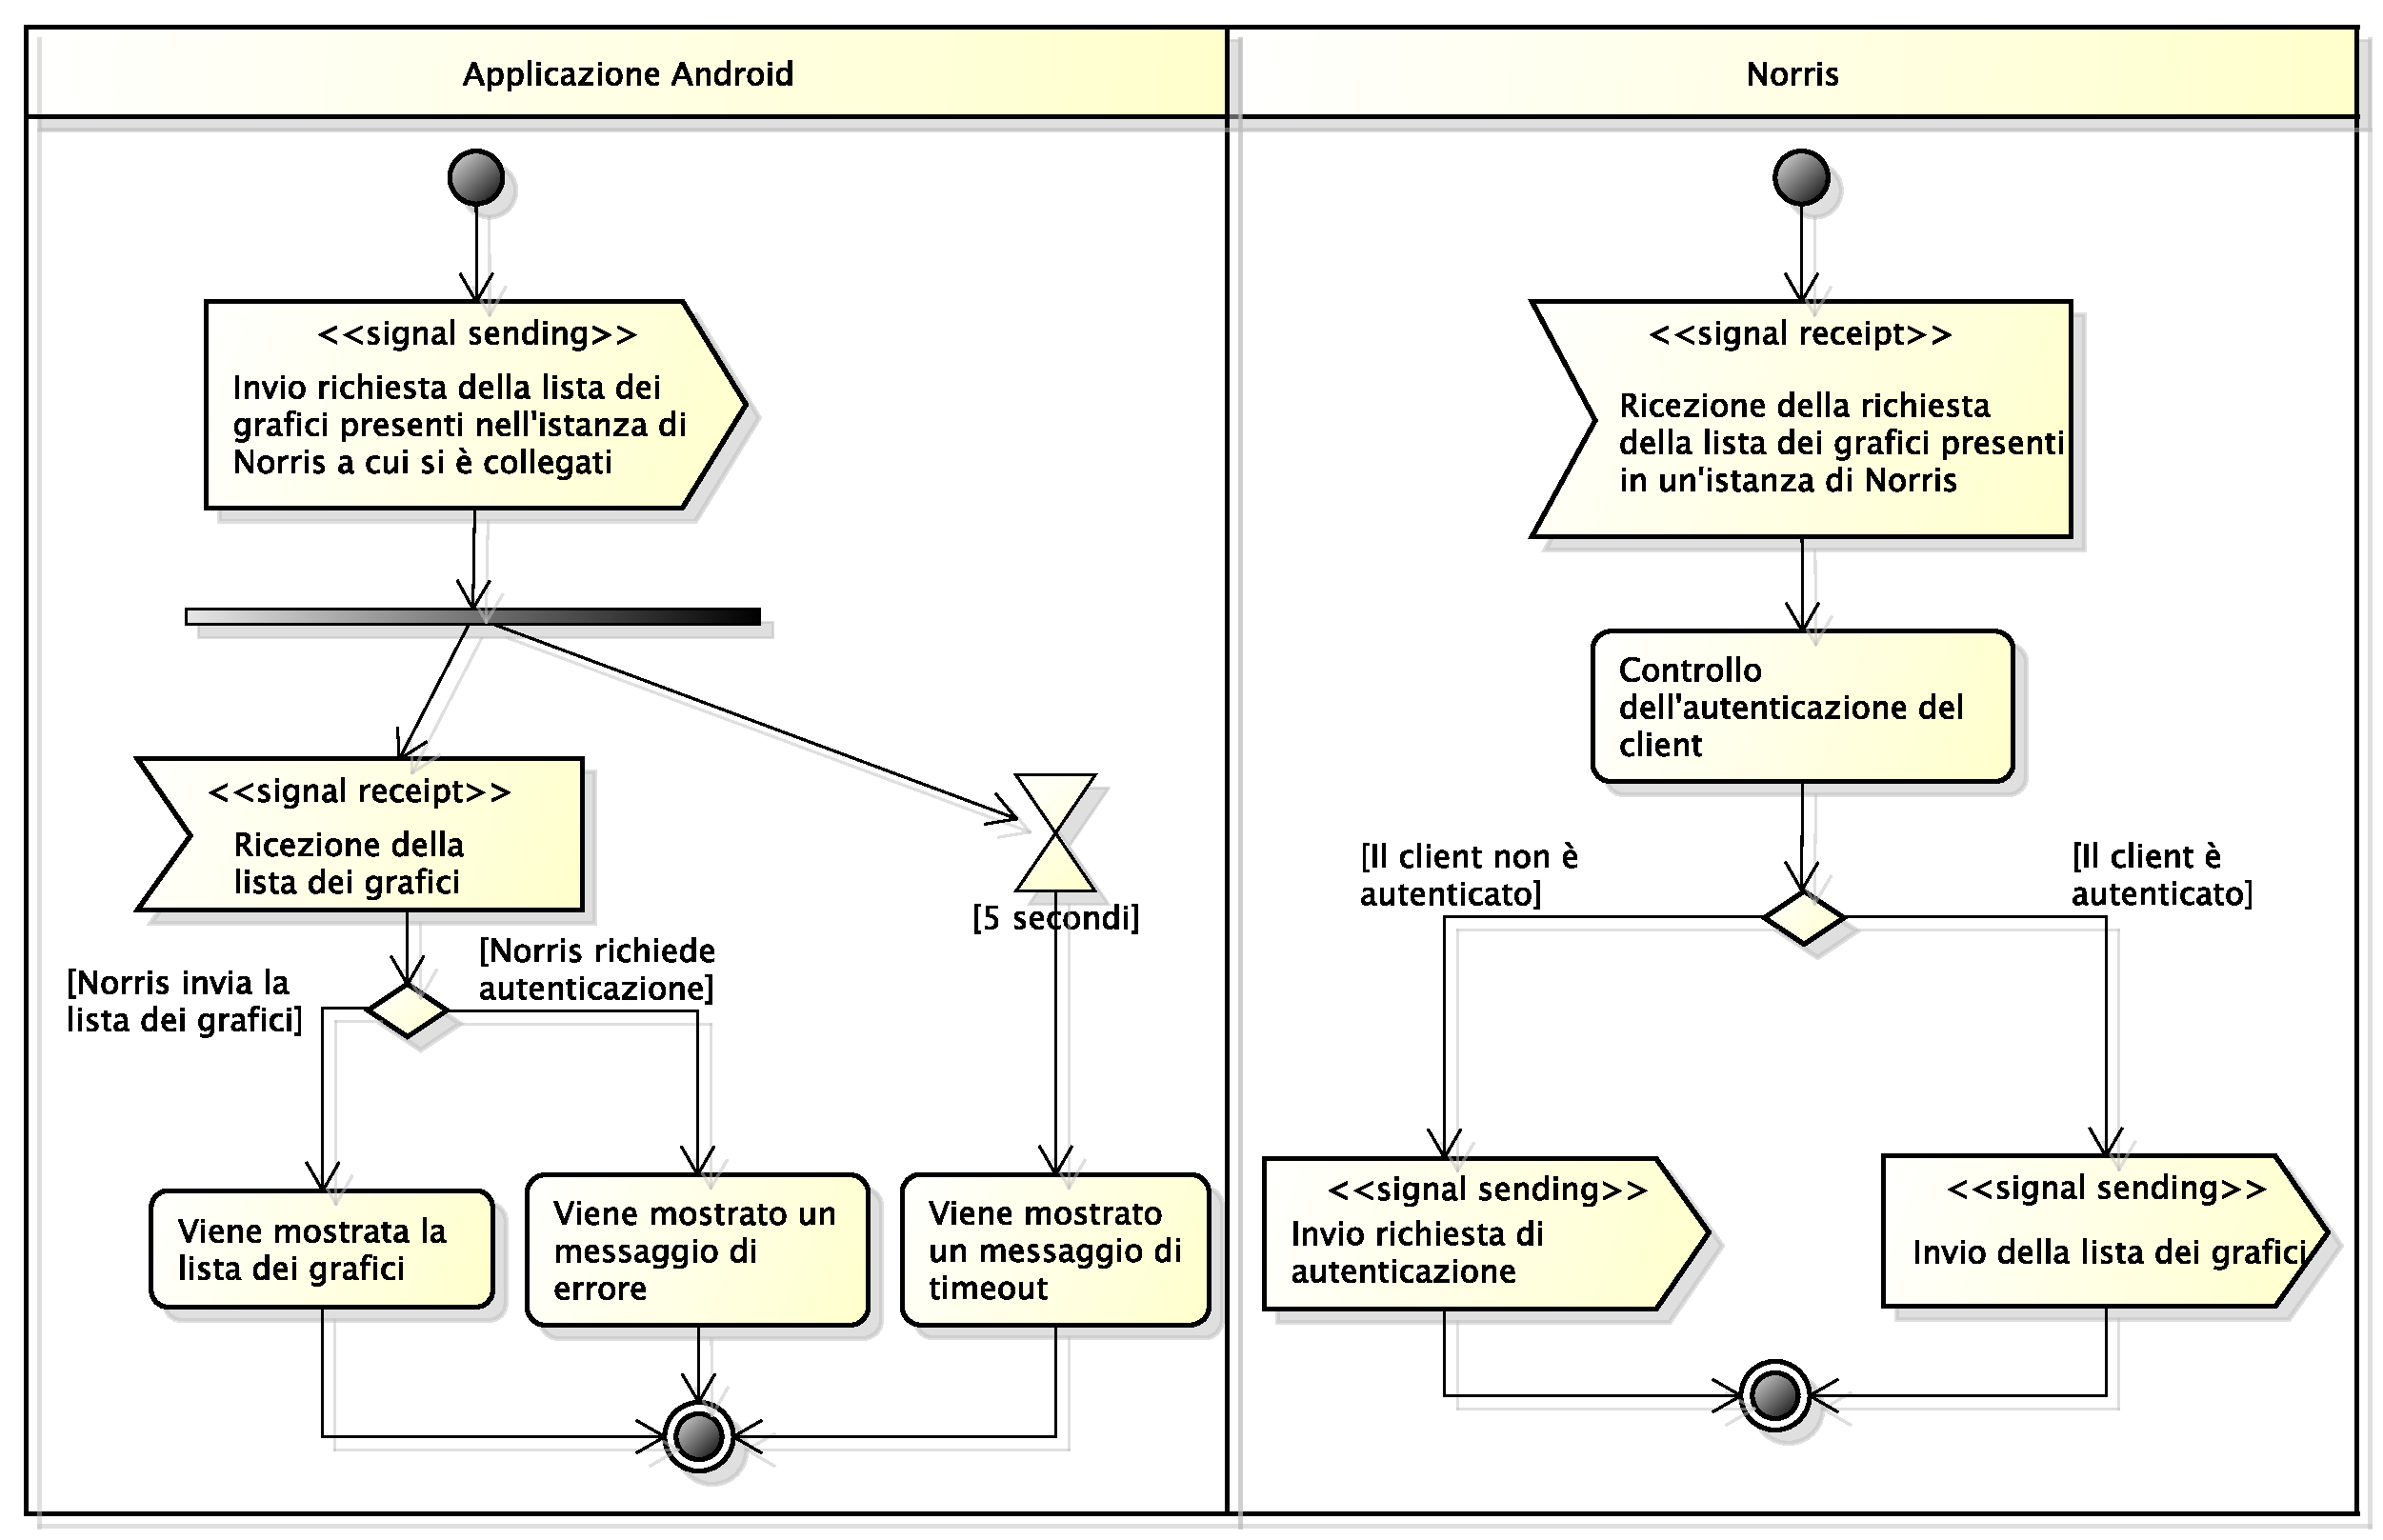
\includegraphics[width=\textwidth]{SpecificaTecnica/Pics/Applicazione/RichiestaLista.pdf}
        	\caption{Diagramma di attività della richiesta delle informazioni di una lista di grafici}
    		\end{figure}
            \item Richiesta informazioni di un grafico: l'applicazione Android manda a Norris una richiesta di informazioni inerenti al grafico che si vuole visualizzare nell'applicazione. Norris controlla se il client è autenticato e, in caso affermativo, manda le informazioni relative al grafico richiesto aprendo una comunicazione tramite websocket. Il canale viene chiuso quando il grafico o l'applicazione sono in background. Riportiamo di seguito un diagramma esplicativo:
            \begin{figure}[H]\centering
        	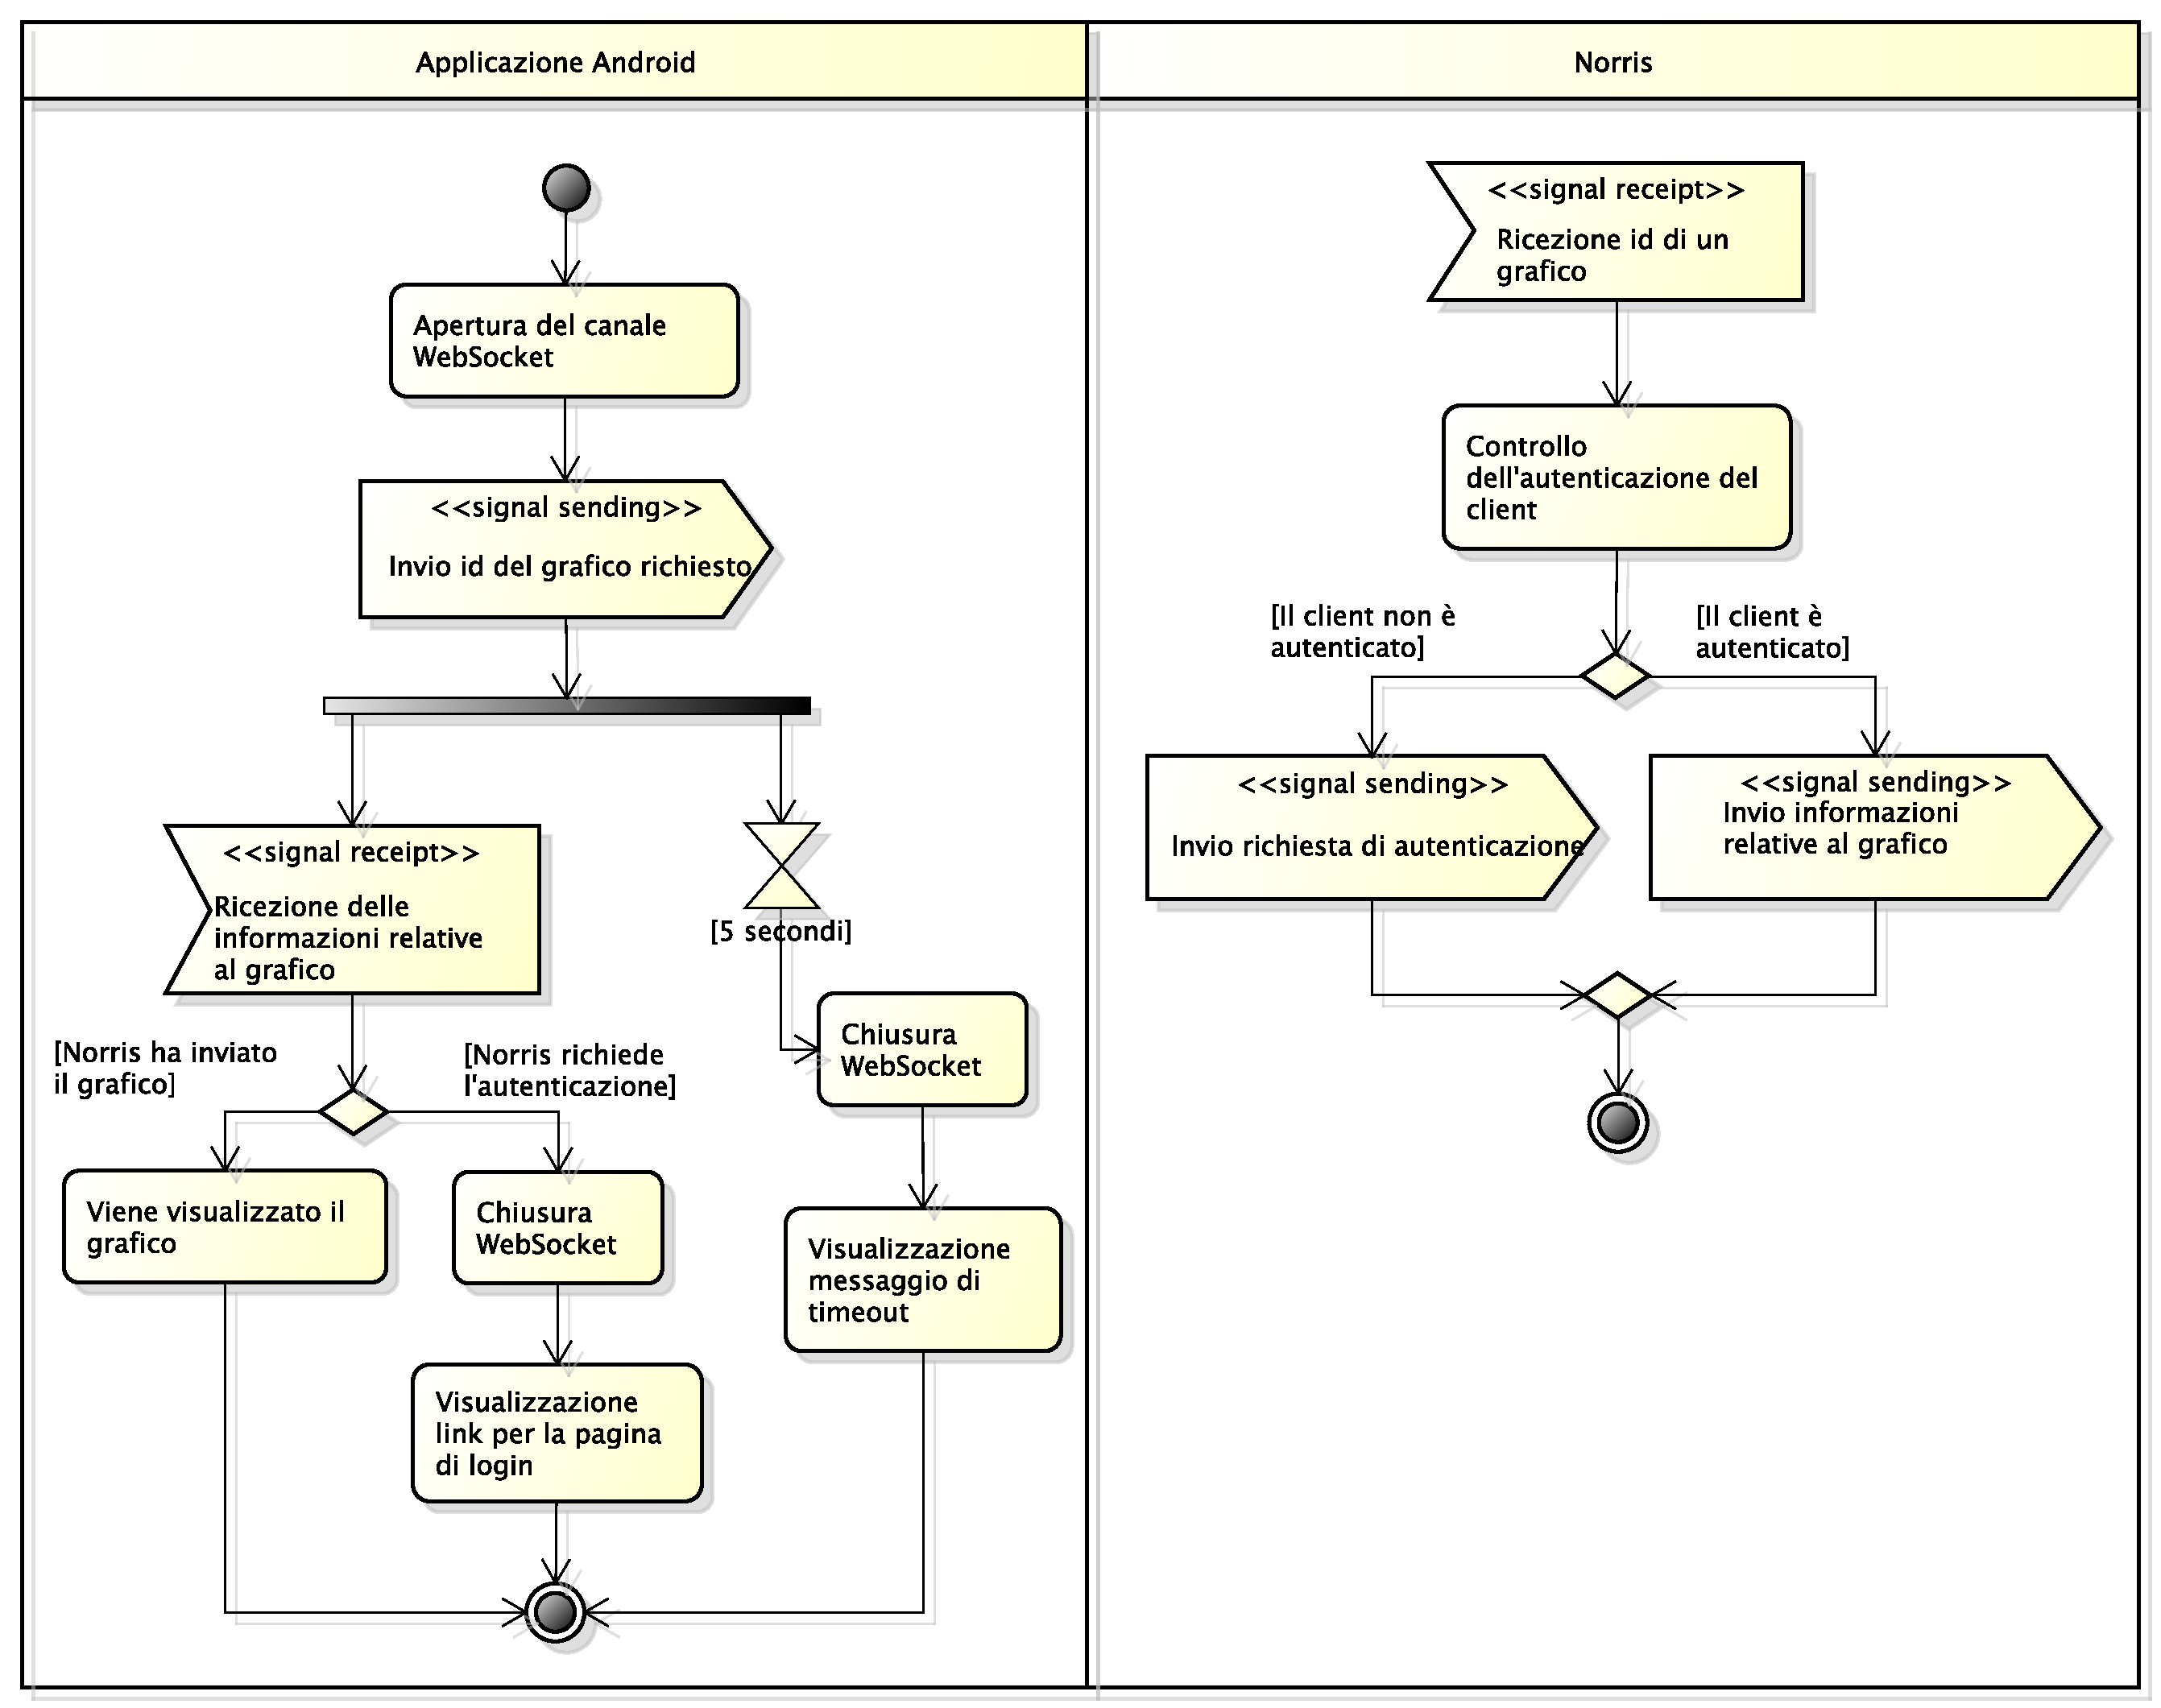
\includegraphics[width=\textwidth]{SpecificaTecnica/Pics/Applicazione/RichiestaGrafico.pdf}
        	\caption{Diagramma di attività della richiesta delle informazioni di un grafico}
    		\end{figure}
            \item Aggiornamenti del grafico: quando un grafico viene aggiornato lato server, Norris si preoccupa di mandare l'aggiornamento ai client che hanno quel grafico. La comunicazione dell'aggiornamento avviene tramite un canale websocket appositamente creato al momento dell'invio dell'aggiornamento. Il canale viene chiuso quando il grafico o l'applicazione sono in background. Gli aggiornamenti avranno luogo solo quando il grafico è attivo. Se il grafico è in background, gli aggiornamenti vengono ignorati. Riportiamo di seguito un diagramma esplicativo:
            \begin{figure}[H]\centering
        	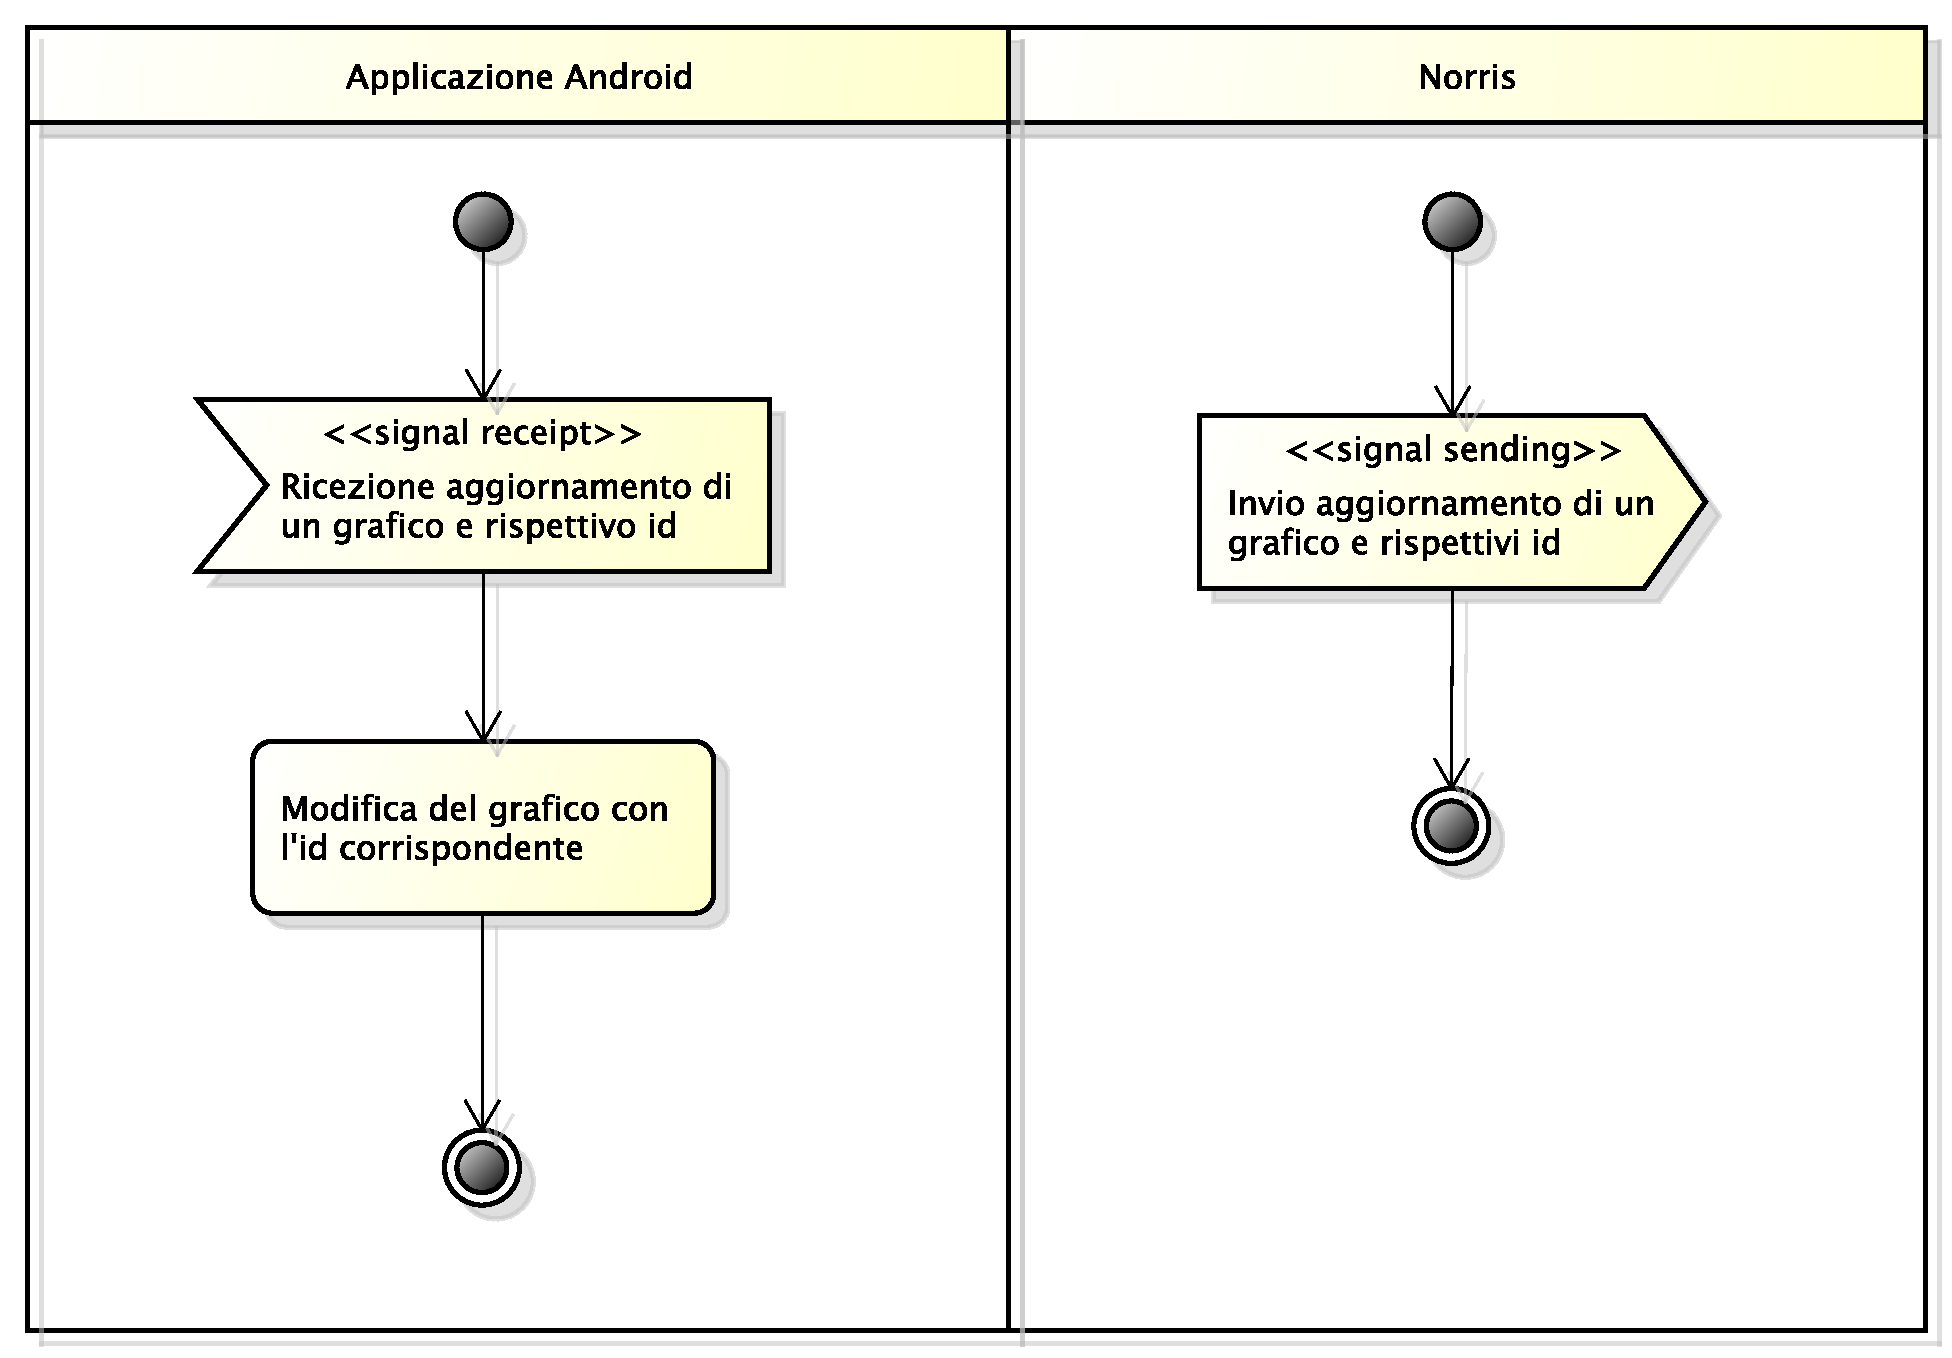
\includegraphics[width=\textwidth]{SpecificaTecnica/Pics/Applicazione/AggiornamentiGrafico.pdf}
        	\caption{Diagramma di attività dell'aggiornamento di un grafico}
    		\end{figure}
        \end{itemize}
